%%%% Paramétrage du TD %%%%
\def\xxactivite{ \ifprof \normalsize{Activation 1 -- Corrigé } \else  \ifcolle Colle \else Activation 1\fi \fi} % \normalsize \vspace{-.4cm}
\def\xxauteur{\textsl{Xavier Pessoles}}


\def\xxnumchapitre{Chapitre 2 \vspace{.2cm}}
\def\xxchapitre{\hspace{.12cm} Hyperstatisme}



\def\xxcompetences{%
\textsl{%
\textbf{Savoirs et compétences :}\\
\begin{itemize}[label=\ding{112},font=\color{ocre}] 
\item \textit{Mod2.C34} : chaînes de solides.
%\item \textit{Mod2.C34} : degré de mobilité du modèle;
%\item \textit{Mod2.C34} : degré d’hyperstatisme du modèle;
%\item \textit{Mod2.C34.SF1} : déterminer les conditions géométriques associées à l’hyperstatisme;
%\item \textit{Mod2.C34} : résoudre le système associé à la fermeture cinématique et en déduire le degré de mobilité et d’hyperstatisme.
\end{itemize}
}}

\def\xxtitreexo{Conception de la commande d’un robot chirurgical}
\def\xxsourceexo{\hspace{.2cm} \footnotesize{CCS PSI 2015}}


\def\xxfigures{
%\includegraphics[width=.7\linewidth]{axe_y_photo}
}%figues de la page de garde


\input{\repRel/Style/pagegarde_TD}
\setcounter{numques}{0}
\setlength{\columnseprule}{.1pt}
\pagestyle{fancy}
\thispagestyle{plain}
\vspace{5.2cm}

\def\columnseprulecolor{\color{ocre}}
\setlength{\columnseprule}{0.4pt} 

%%%%%%%%%%%%%%%%%%%%%%%

\setcounter{exo}{0}
\ifprof
\else

\ifprof
\begin{multicols}{2}
\else
\begin{multicols}{2}
\fi


On s'intéresse au bras esclave d'un robot chirurgical. 
\begin{obj}
Justifier la structure du bras esclave par rapport au cahier des charges.
\end{obj}

\begin{center}
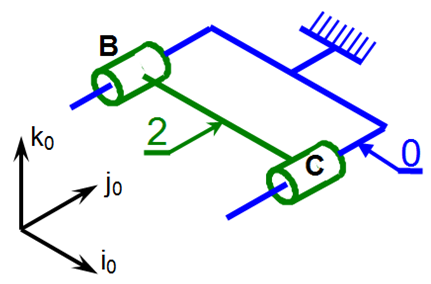
\includegraphics[width=\linewidth]{fig_02.png}
\end{center}

On donne le schéma cinématique partiel du bras esclave.

\begin{center}
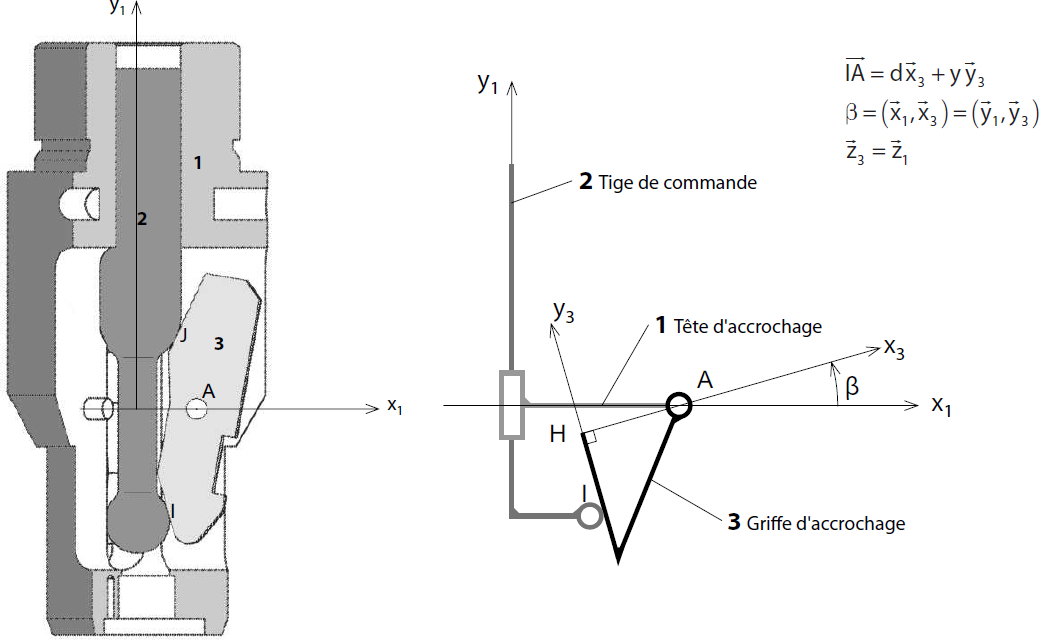
\includegraphics[width=\linewidth]{fig_01.png}
\end{center}

\begin{center}
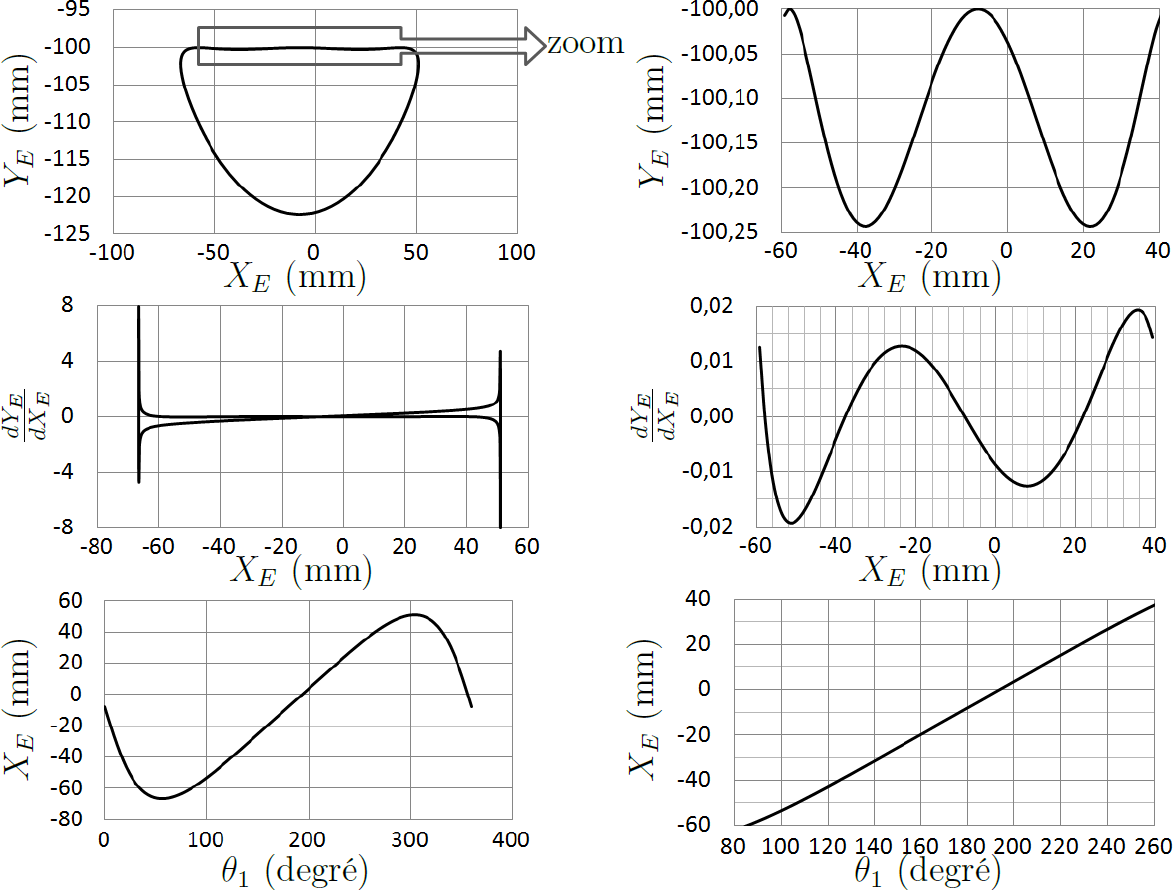
\includegraphics[width=\linewidth]{fig_03.png}
\end{center}


\begin{center}
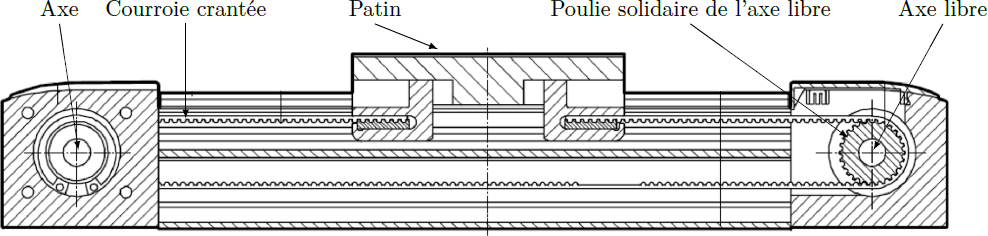
\includegraphics[width=\linewidth]{fig_04.png}
\end{center}

Le point $T$ est situé à l’intersection des axes $\axe{A'}{{x_0}}$ et  $\axe{P'}{{y_2}'}$. 
Le vecteur vitesse du point $T$ de 7’ par rapport à 0, noté $\vectv{T}{7'}{0}$, doit être colinéaire à 
$\vect{y_2}'$.

\question{Tracer le graphe de liaison.}

\question{En s’appuyant sur le schéma cinématique, calculer $\vectv{P}{7'}{0}$ par dérivation du vecteur position.}

\question{Exprimer $\vectv{T}{7'}{0}$ dans la base $\base{x_2'}{y_2'}{z_2'}$ en fonction des données de l’énoncé. Il est conseillé d’utiliser la relation de Varignon en passant par le point $P'$.}


\question{Exprimer le torseur cinématique de $7’/0$ réduit en $T$, par ses composantes dans la base $\base{x_2'}{y_2'}{z_2'}$ et donner la liaison équivalente entre 7’ et 0 au point $T$.}


\question{Quelle exigence du cahier des charges (document réponse) justifie cette structure ? Expliquer sans calcul.}

\question{Mettre à jour le graphe de liaisons et donner le degré d'hyperstatisme du modèle. Vous utiliserez la méthode statique et la méthode cinématique.}

\question{Quel peut être l'avantage de disposer d'un système hyperstatique ?}

\question{En conservant l'architecture du mécanisme, proposer des modifications de liaisons permettant de rendre le modèle isostatique.}



\ifprof
\end{multicols}
\else
\end{multicols}
\fi




